%%%%%%%%%%%%%%%%%%%%%%%%%%%%%%%%%%%%%%%%%%%%%%%%%%%%%%%%%%%%%%%%%%%%
%% I, the copyright holder of this work, release this work into the
%% public domain. This applies worldwide. In some countries this may
%% not be legally possible; if so: I grant anyone the right to use
%% this work for any purpose, without any conditions, unless such
%% conditions are required by law.
%%%%%%%%%%%%%%%%%%%%%%%%%%%%%%%%%%%%%%%%%%%%%%%%%%%%%%%%%%%%%%%%%%%%

\PassOptionsToPackage{
  plainpages = false,               								
  pdfpagelabels,
  unicode,  
  colorlinks = true,
  linkcolor = link-grey,	% PC version
  citecolor = crimson,		% PC version
  urlcolor = blue,			% PC version
  % linkcolor = black,		% Print version
  % citecolor = black,		% Print version
  % urlcolor = black,		% Print version
}{hyperref}

\documentclass[
  digital,  	% PC version
  color,		% PC version
  oneside,   	% PC version
  % printed 	% Printed version
  % monochrome	% Printed version
  % twoside		% Printed version
  12pt,
  nocover,
  notable,
  nolof,
  nolot,
  %% More options are listed in the user guide at
  %% <http://mirrors.ctan.org/macros/latex/contrib/fithesis/guide/mu/fi.pdf>.
]{fithesis3}

%% The following section sets up the locales used in the thesis.
\usepackage[resetfonts]{cmap} %% We need to load the T2A font encoding
\usepackage[utf8]{inputenc}
\usepackage[T1,T2A]{fontenc}  %% to use the Cyrillic fonts with Russian texts.
\usepackage[
  main=english,
  english, german, russian, czech, slovak
]{babel}
%% fonts:
\usepackage{paratype}
\def\textrussian#1{{\usefont{T2A}{PTSerif-TLF}{m}{rm}#1}}

%%\shorthands{off}
%% The following section sets up the metadata of the thesis.
\thesissetup{
    date          = \the\year/\the\month/\the\day,
    university    = mu,
    faculty       = fi,
    type          = mgr,
    author        = Ľubomír Obrátil,
    gender        = m,
    advisor       = {RNDr. Petr Švenda, Ph.D.},
    title         = {Randomness Testing Toolkit},
    TeXtitle      = {The automated testing of randomness with multiple statistical batteries},
    keywords      = {TODO},
    TeXkeywords   = {TODO},
    abstract      = {TODO},
    thanks        = {TODO},
    bib           = bibliography.bib,
}
\usepackage{makeidx}      %% The `makeidx` package contains
\makeindex                %% helper commands for index typesetting.
\thesisload


\newcommand{\lmar}{3.6cm} % PC
\newcommand{\rmar}{3.6cm} % PC
%\newcommand{\lmar}{4cm} % Printed
%\newcommand{\rmar}{3.2cm} % Printed

\usepackage[top=3cm, bottom=3.5cm, left=\lmar, right=\rmar]{geometry}

%% These additional packages are used within the document:
\usepackage{minted}
\usepackage{paralist} %% Compact list environments
\usepackage{amsmath}  %% Mathematics
\usepackage{amsthm}
\usepackage{url}
\usepackage{enumitem}
\usepackage{amsfonts}
\usepackage{markdown} %% Lightweight markup
\usepackage{dirtree}

\usepackage{xcolor}
\definecolor{link-grey}{rgb}{0.3,0.3,0.3}
\definecolor{code-bg-grey}{rgb}{0.85,0.85,0.85}
\definecolor{code-bg-light_grey}{rgb}{0.92,0.92,0.92}
\definecolor{crimson}{rgb}{0.6,0,0}

% Eliminates margins
\def\nomar{\list{}{\rightmargin-\rmar\leftmargin-\lmar}\item[]}
\let\endnomar=\endlist

% Various macros
\setlength{\parskip}{0.5em}
\setlist[description]{leftmargin=0cm , itemsep = 0cm}
\setlist[itemize]{noitemsep}

% Itemize with title
\newenvironment{titlemize}[1]
{
	\begin{description}
	\item[#1]\
	\begin{itemize}
}
{
	\end{itemize}
 	\end{description}
}

% Let tables and figures share numbering
\makeatletter \let\c@table\c@figure \makeatother

%%%%%%%%%%%%%%%%%%%%%%%%%%%%%%%%%%%%%%%%%%%%%%%%%%%%%%%%%%%%%%%%%%%%%%%%%%%%%%%%%%%%%%%%
%%%%%%%%%%%%%%%%%%%%%%%%%%%%%%%%%%%%%%%%%%%%%%%%%%%%%%%%%%%%%%%%%%%%%%%%%%%%%%%%%%%%%%%%
% =================================== TEXT BEGINNING =================================== 
%%%%%%%%%%%%%%%%%%%%%%%%%%%%%%%%%%%%%%%%%%%%%%%%%%%%%%%%%%%%%%%%%%%%%%%%%%%%%%%%%%%%%%%%
%%%%%%%%%%%%%%%%%%%%%%%%%%%%%%%%%%%%%%%%%%%%%%%%%%%%%%%%%%%%%%%%%%%%%%%%%%%%%%%%%%%%%%%%
% Final Description:
%The randomness and pseudorandomness are important security property of output of a random number generator as well a cryptographic function. To some extent, these characteristics can be measured and tested by randomness statistical batteries like STS NIST or DIEHARDER. The thesis is aimed at development of a tool that would provide means for fast, simple and consistent testing of randomness of arbitrary data using multiple statistical batteries.

%The thesis will provide an introduction to statistical randomness testing and interpretation of results obtained from a given test and battery. The toolkit for easy remote execution of statistical tests on a dedicated server will be developed with the following functionality:

% - Easy submission of data for testing, both locally (filesystem) and remotely (web interface)
% - At least three different statistical batteries will be incorporated via unified interface
% - Unified presentation of test results of executed batteries
%The tool will be utilized in subsequent experiments aimed to compare classical batteries with EACirc framework and also evaluate test behavior of DIEHARDER on large amount of truly random data.

%Literature
%STS NIST battery, http://csrc.nist.gov/groups/ST/toolkit/rng/index.html [2017-03-13]
%R. Brown, Dieharder battery, https://www.phy.duke.edu/~rgb/General/dieharder.php[2017-03-13]

\begin{document}

\chapter{Introduction}
\begin{itemize}
\item Randomness, why should we test it (defects, low entropy, etc...)
\item Statistical testing of randomness
\end{itemize}

\chapter{Used third-party statistical software}
\label{chap:batteries}
In this chapter, we will explain terminology specific to Randomness Testing Toolkit; present a quick overview of the statistical software used in the toolkit and describe the observed and unexpected behavior of the statistical software in edge cases. We also list undertaken measures to mitigate the undocumented behaviour in our further experiments.

\section{Terminology}
Throughout the thesis, we are using certain expressions in the context of Randomness Testing Toolkit and the tools and math it uses. We list these terms along with their explanations here.

\begin{description}
\item[(Statistical) Battery] \hfill \\
A program developed by a third party serving as a tool for evaluation of randomness of arbitrary binary data. A statistical battery usually contains one or multiple statistical tests. The final result of the assessment is based on the results of the tests. Examples of statistical batteries are NIST Statistical Test Suite, Dieharder or TestU01.

\item[(Statistical) Test] \hfill \\
A single unit in statistical battery that measures some property of the tested binary stream (e.g. number of zeroes). The test can have multiple variants and subtests, and the result of the test is one or multiple statistics.

\item[Null hypothesis - $H_0$] \hfill \\
The hypothesis $H_0$ denotes the hypothesis that the tested data stream is random. Based on the results of the test, we can either reject $H_0$ and say that the data is not random or not reject it. In the latter case, we assume that the tested data is indeed random.

\item[P-value] \hfill \\
In our hypothesis testing, a p-value is a probability of obtaining equal or more extreme test result while $H_0$ holds true. In our situation, a p-value denotes the probability that we would get same or more extreme test results when testing truly random data. Therefore, the closer the p-value is to 0 the less is the probability the tested data is random and vice versa.

\item[Alpha - $\alpha$] \hfill \\
Significance level based on which we either reject or not reject $H_0$. We can specify some interval (e.g. $[0,\alpha]$) and if the result of the test (p-value) falls into this interval, we will reject the hypothesis that the tested data is random. Alternatively, we can also reject p-values that are too extreme on both sides of the interval (outside of $\left[\frac{\alpha}{2},1-\frac{\alpha}{2}\right]$).

\item[Statistic] \hfill \\
The value obtained by certain calculation from first level p-values. Multiple statistics can be obtained from one set of p-values e.g. when testing the set for uniformity we can use Kolmogorov-Smirnov Test or Chi-Square test. Based on values of statistics of a test we can decide rejection of $H_0$.

\item[Test sample] \hfill \\
A single execution of a statistical test. The result of single test execution is one first level p-value. By repeating execution of the test, we obtain multiple p-values. By using a certain statistic (e.g. Kolmogorov-Smirnov test), we can calculate a single second level p-value.

\item[Variant of a test] \hfill \\
Many tests can be parametrized in some ways, possibly giving different results with the same input data. We don't treat multiple executions of a single test with different settings as separate units but rather as variants of that test.

\item[Subtest] \hfill \\
Some tests, even when executed only once, may measure multiple properties of the data thus providing multiple results. For example, Serial Test from Dieharder battery will measure frequencies of all 1, 2, .., 16-bit patterns in the data. We treat these measurements separately - as subtests of the test. Subtests can have multiple separate statistics.

\item[Job] \hfill \\
Single execution of Randomness Testing Toolkit that will analyse single binary data file with single statistical battery.

\item[Experiment] \hfill \\
Batch of jobs that analysed single data file with various statistical batteries and settings.

\end{description}

\section{Batteries supported by RTT}
\subsection{NIST Statistical Test Suite}
The battery of statistical tests was developed by National Institute of Standards and Technology (cit.). The battery implements 15 statistical tests for evaluating randomness of input data.

The reference implementation is not used in RTT because it is considerably slower than its optimized counterparts. The faster version of NIST STS used in RTT was developed by Zdeněk Říha and Marek Sýs(cit.). 

\subsection{Dieharder}
Dieharder is a battery designed by Robert G. Brown at the Duke University (cit.). The battery features user-friendly console interface with the possibility of fine-grain modification of the test parameters. The fact that Dieharder is included in repositories of some Linux distributions (cit manpage) adds to its popularity and ease of use. Dieharder includes all tests from the older statistical battery Diehard (cit.), three tests from NIST STS and several other tests implemented by the author. 

Since the original Dieharder implementation doesn't output all of the information we needed for interpretation and evaluation of the results, we had to modify the source code of the battery. RTT uses this modified Dieharder.

\subsection{TestU01}
This library of statistical batteries was developed at Université de Montréal by Pierre L’Ecuyer et al. (cit.). It contains a wide range of tests from NIST STS, Dieharder, and literature. It also implements various pseudo-random number generators. The statistical tests are grouped into multiple categories each intended for different use-case scenario. We will treat these categories of tests as separate batteries. TestU01 includes following ten batteries.
\begin{description}
\item[Small Crush, Crush, Big Crush] \hfill \\
Small Crush battery is very fast and needs a relatively small amount of data to run - around 250 megabytes. Small Crush is also the only battery that can be natively used for analysis of data in a binary file, for the use of Crush and Big Crush, the user has to implement PRNG with the TestU01 interface. Crush and Big Crush batteries are more stringent and need gigabytes of data and a few hours to finish while Big Crush is more time and data demanding.
\item[Rabbit, Alphabit, Block Alphabit] \hfill \\
Tests in these batteries are suited for testing hardware bit generators and can be applied to an arbitrary amount of data. Data can be provided either as a binary file or PRNG implementing the TestU01 interface.
\item[PseudoDIEHARD, FIPS\_140\_2] \hfill \\
Tests in PseudoDIEHARD imitate DIEHARD battery; FIPS\_140\_2 battery implements a small suite of tests in NIST standard(cit.) Randomness Testing Toolkit doesn't support these two batteries since they are subsets of other supported batteries.
\end{description}

Since TestU01 is available only as an ANSI C library, we developed a console interface for it. The interface implements a dummy number generator that provides data from a supplied binary file to the battery. Our interface allows us to apply batteries to arbitrary binary data even when the batteries don't support this feature natively.

\section{Unexpected behavior and errors of the batteries}
To examine the boundary behavior of the above-listed tools, we used them to process extremely non-random data streams. The data streams that we used as the input to the batteries were two binary data files consisting of only zeroes and ones respectively. The settings of the batteries remained set to default. 

Below we list observed undocumented behavior that differs from the execution of the batteries with non-extreme input.

\subsection*{NIST Statistical Test Suite}
Each test in the battery processed 1000 separate data streams. Each data stream was 1000000 bits long.

Tests Random Excursions and Random Excursions Variant are not applicable to all possible data streams. In a regular run with reasonably random data, this doesn't matter much, as the tests are repeated multiple times, and the final result will simply be calculated from a lesser number of p-values. 

Neither of the tests can be applied to a stream full of zeroes or ones. This causes absence of results when analyzing such data. The user can find out the fact that the tests are not applicable to provided stream after he inspects logs of the program; otherwise, the interpretation of the missing results is left to him.

\subsection*{Dieharder}
When processing extremely non-random data with Dieharder, we observed various erroneous events. The events are summarized in Table~\ref{tab:dieharder_errors}. 

\begin{table}[h!]
\begin{nomar}
\centering
\begin{tabular}{ l || c | c }
\textbf{Test name}                   & \textbf{Stream of zeroes} & \textbf{Stream of ones} \\ \hline \hline
STS Runs                             & No result                & No result                \\ \hline
DAB Monobit 2 						 & Invalid result           & Invalid result           \\ \hline
Diehard Minimum Distance (2D Circle) & Stuck execution          & -                        \\
Diehard 3D Sphere (Minimum Distance) & Stuck execution          & -                        \\
Marsaglia and Tsang GCD              & Stuck execution          & -                        \\
RGB Generalized Minimum Distance     & Stuck execution          & -                        \\
RGB Kolmogorov-Smirnov               & Stuck execution          & -                        \\  
Diehard Craps                        & -                        & Stuck execution          \\
RGB Bit Distribution                 & -                        & Stuck execution          \\
\end{tabular}
\end{nomar}
\caption{Undocumented behavior of tests in Dieharder battery}
\label{tab:dieharder_errors}
\end{table}

\begin{titlemize}{Observed errors}
\item \textbf{No result} Test didn't provide any p-values that would be used to calculate the final result of the test. The user is not notified of this, and the final result of the test statistic is based on default value (1.0).
\item \textbf{Invalid result} Test provided resulting statistic and there was no indication of error other than that the result was again default value of the statistic (1.0). Following the definition of p-value, the interpretation of such result is that the analyzed stream was almost certainly random. This is obviously not true, as both streams are just repeating ones or zeroes respectively. 
\item \textbf{Stuck execution} Tests froze at a certain point in execution, did not produce any results and we were forced to kill the processes manually.
\end{titlemize}

\subsection*{TestU01}
Batteries Small Crush, Crush, Big Crush, Rabbit, Alphabit and Block Alphabit were executed. Tests that are part of multiple batteries acted in the same way across the batteries. The behavior is summarized in Table~\ref{tab:testu01_errors}.

\begin{table}[h!]
\begin{nomar}
\centering
\begin{tabular}{l || c | c }
\textbf{Test name}                 & \textbf{Stream of zeroes} & \textbf{Stream of ones} \\ \hline \hline    
sstring\_Run                       & No result                & No result                \\
sknuth\_Gap                        & No result                & -                        \\ \hline
svaria\_SampleProd                 & All results invalid      & All results invalid      \\
svaria\_AppearenceSpacings         & All results invalid      & All results invalid      \\   
scomp\_LinearComp                  & All results invalid      & All results invalid      \\
scomp\_LempelZiv                   & All results invalid      & All results invalid      \\
svaria\_SampleCorr                 & -                        & All results invalid      \\ \hline
sknuth\_MaxOft                     & Some results invalid     & Some results invalid     \\
svaria\_SampleMean                 & Some results invalid     & Some results invalid     \\
sspectral\_Fourier3                & Some results invalid     & Some results invalid     \\
sstring\_HammingWeight2            & Some results invalid     & Some results invalid     \\
sstring\_AutoCor                   & Some results invalid     & Some results invalid     \\
smultin\_MultinomialBitsOver       & Some results invalid     & Some results invalid     \\
sstring\_LongestHeadRun            & -                        & Some results invalid     \\ \hline
snpair\_ClosePairs                 & Stuck execution          & Stuck execution          \\
snpair\_ClosePairsBitMatch         & -                        & Stuck execution          \\
svaria\_SumCollector               & -                        & Stuck execution          \\
smarsa\_GCD                        & -                        & Stuck execution          \\                                       
\end{tabular}
\end{nomar}  
\caption{Undocumented behavior of tests in TestU01 library}
\label{tab:testu01_errors}                                                                                           
\end{table}

\begin{titlemize}{Observed errors}
\item \textbf{No results} Tests reported warning and ended without any result. This is probably caused by the tests not being applicable to provided data.
\item \textbf{All results invalid}  All statistics of the test reported p-value very close to 1.0. This could lead the user to the interpretation that the test reports the data as an almost perfect random stream.
\item \textbf{Some results invalid} Similar situation to the previous one but not all statistics of the test are close to 1.0. Results of tests statistics are either close to 0.0 or 1.0.
\item \textbf{Stuck execution} Tests froze at a certain point of execution. In some cases, this is preceded by an issued warning. Tests didn't produce any results and had to be killed manually.
\end{titlemize}

\subsection{Preventive measures in RTT}
Since we need to use the batteries in RTT with arbitrary binary data, we implemented following measures that mitigate above-mentioned errors in our experiments.
\begin{itemize}
\item Tests that don't produce any results are ignored and treated as if never executed.
\item Because some tests give 1.0 as a result of their statistics when the data are clearly not random, we will reject the hypothesis of randomness either when the p-value is too close to 0 or too close to 1. More specifically, $H_0$ will be rejected for all p-values that falls outside of the interval $\left[\frac{\alpha}{2}, 1-\frac{\alpha}{2}\right]$. This way we reject all results that are too extreme.
\item Each test is executed with the timeout. If the test doesn't finish within defined time limit, we will automatically terminate it and then treat it as if it didn't produce any results.
\end{itemize}

\chapter{Randomness Testing Toolkit}
%\begin{itemize}
%\item Motivation - unified interface to batteries, ease of use, unified result format/representation
%\item Local execution of RTT - battery and toolkit configuration, installation, brief implementation and interface overview - more thorough in documentation and comments
%\item Local result format - either database or file output storage
%\item Remote execution of RTT - toolkit deployed on server infrastructure, system overview (database, frontend, backend(s), storage), accessible through ssh on limited system or via web interface (django), results in database
%\item Remote results of RTT - email notification, webpage layout
%\item Interpretation of results of RTT
%\begin{itemize}
%\item Grouping subtests together - eliminating intertest bias
%\item How grouping works - theory, Sidak correction, partial p-value, fail/pass of a test
%\end{itemize}
%\end{itemize}
One of our goals during working in this project was to create a tool that would provide fast and user-friendly analysis of randomness even for users not experienced in the field of statistical randomness testing. Process of statistical testing generally includes finding a suitable tool, installation of said tool, execution and interpretaion of the analysis.

Another motivation was that the developed tool would unify the process of randomness analysis that is often done by reserachers in CRoCS\footnote{Centre for Research of Cryptography and Security}. Before the start of the project, each researcher used his own set of scripts and tools which is difficult to manage and also complicates comparation of the experiments done by different people.

Therefore we developed Randomness Testing Toolkit\footnote{Also referenced as RTT or just the toolkit.} that serves as an unified interface of the three statistical batteries presented in Chapter~\ref{chap:batteries}. The toolkit consists of several connected parts that are intended for various purposes. Apart from interfaces and data storage format, the parts are independent and can be exchanged if needed.

In following sections of this chapter, we will provide detailed description of the implemented parts of the toolkit.

\section{Local unified interface}
The local unified interface is at the lowest level of the developed parts of RTT. The interface is a binary executable that accepts settings and outputs the results in common format for all batteries. The executable handles transformation of general settings into the battery specific ones, running the battery executable and then transforming gathered output into general format. The process is visualized in Figure~\ref{fig:rtt_local_workflow}.

The toolkit accepts settings needed for its run from three following sources:
\begin{itemize}
\item \textbf{Command-line arguments} -- Basic settings that change for each run, for example path to input file with binary data or to file with battery configuration.
\item \textbf{Toolkit settings file} -- General settings for the toolkit related to the system environment e.g. paths to executables of the statistical batteries. In most cases the settings stay the same for all executions of the toolkit regardless of the battery or data used.
\item \textbf{Battery configuration file} -- Configuration file that fully configures input settings for single or multiple batteries. The configuration of the batteries can change between the executions of the toolkit.
\end{itemize}

\begin{figure}[h!]
\begin{nomar}
\centering
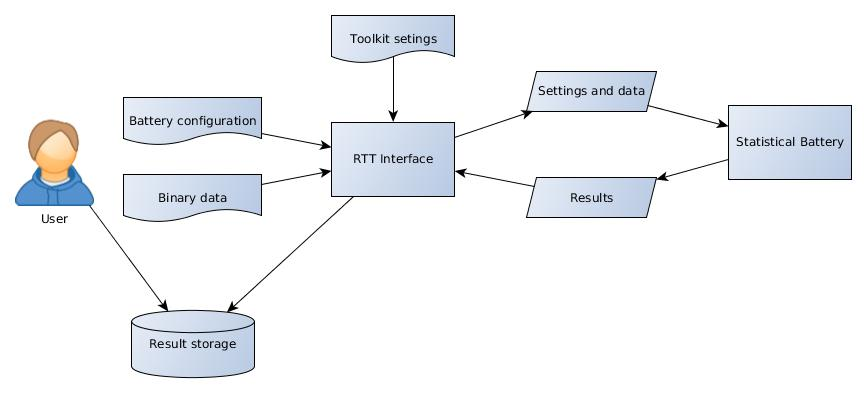
\includegraphics[width=\paperwidth-4cm]{figures/local-rtt-workflow.jpg}
\end{nomar}
\caption{Local RTT workflow}
\label{fig:rtt_local_workflow}
\end{figure}

\subsection{Command-line arguments}
The basic options of the RTT execution are set through command-line arguments. RTT recognizes following options.

\begin{itemize}
\item \texttt{-h} Usage of the toolkit will be printed.
\item \texttt{-b <battery>} Sets the battery that will be executed during the run. Values accepted as \texttt{<battery>}: dieharder, nist\_sts, tu01\_smallcrush, tu01\_crush, tu01\_bigcrush, tu01\_rabbit, tu01\_alphabit and tu01\_blockalphabit.
\item \texttt{-t <test-id>} Optional argument. If set, only single test with id \texttt{<test-id>} will be executed in the battery.
\item \texttt{-c <config-path>} Path to file with configuration of the battery. Details about battery configuration are in Section~\ref{sec:batt_conf}.
\item \texttt{-f <data-path>} Path to file with the binary data that will be analyzed by the executed battery.
\item \texttt{-r <result-storage>} Sets the type of the result storage that will be used. Accepted values are \texttt{file-report} or \texttt{db-mysql}. The option doesn't have to be set; \texttt{file-report} is then used as default option. More information about result storages is in Section~\ref{sec:result_storages}.
\item \texttt{-eid <experiment-id>} Option mandatory only when \texttt{db-mysql} is set as result storage, is ignored otherwise. Sets to which experiment in the database will be tied the results of the analysis. 
\end{itemize}

\subsection{Toolkit settings}
The general settings of the toolkit are kept in separate file \texttt{rtt-settings.json} and are related to environment in which the toolkit will be executed (e.g. locations of the files and directories). The file is created by the user after the toolkit installation and stays the same for all subsequent executions of the program unless the environment changes (as opposed to input file with configuration of the batteries that can be different for each data analysis). The file \texttt{rtt-settings.json} must be located in the working directory from which the program is executed.

Basic structure of the file is in Figure~\ref{fig:rtt_sett_short_json}. A complete example file can be found in Appendix~\ref{app:rtt_sett_json}. 

%  {
%    "toolkit-settings": {
%      "logger": {...},
%      "result-storage": {
%        "file": {...},
%        "mysql-db": {...}
%      },
%      "binaries": {...},    
%      "miscelaneous": {
%        "nist-sts": {...}
%      },
%      "execution": {...}
%    }
%  }
\begin{figure}[h!]
\begin{minted}[mathescape,
               linenos,
               numbersep=5pt,
               gobble=2,
               frame=lines,
               framesep=2mm]{json}
  {
    "toolkit-settings": {
      "logger": {
        "comment": "Program logger settings"
      },
      "result-storage": {
        "file": {
          "comment": "File result storage settings"
        },
        "mysql-db": {
          "comment": "MySQL Database storage settings"
        }
      },
      "binaries": {
        "comment": "Executable binaries locations"
      },    
      "miscelaneous": {
        "nist-sts": {
          "comment": "Miscellaneous NIST STS settings"
        }
      },
      "execution": {
        "comment": "Battery execution settings"
      }
    }
  }
\end{minted}
\caption{Basic structure of \texttt{rtt-settings.json}}
\label{fig:rtt_sett_short_json}
\end{figure}

The description of the individual tags and the options that can be set within them follows.

\begin{description}
\item[toolkit-settings/logger] \hfill \\
Tag containing settings related to location of log files produced during runtime.
\begin{itemize}
\item \textbf{dir-prefix} \textit{Optional} -- If set, value of this tag will become prefix of all log locations. Can be used when all logger directories should have same parent directory.
\item \textbf{run-log-dir} -- Sets location of the main log file.
\item \textbf{<battery>-dir} -- Value \textbf{<battery>} is replaced by values dieharder, nist-sts, tu01-smallcrush, tu01-crush, tu01-bigcrush, tu01-rabbit tu01-alphabit and tu01-blockalphabit. All of these tags are mandatory and set locations of files that will contain raw outputs of the respective executed batteries.
\end{itemize}

\item[toolkit-settings/result-storage/file] \textit{Optional} \hfill \\
Section with settings needed for file result storage. All values of tags except tag \textbf{main-file} are treated as directories. For details about the storage see Section~\ref{sec:file_res_storage}.
\begin{itemize}
\item \textbf{main-file} -- Sets path of the file with final results of the program run. If the file already exists, results will be added to it, if not, new result file will be created.
\item \textbf{dir-prefix} -- If set, all directory values will have this prefix.
\item \textbf{<battery>-dir} -- Value \textbf{<battery>} can be replaced by values dieharder, nist-sts, tu01-smallcrush, tu01-crush, tu01-bigcrush, tu01-rabbit, tu01-alphabit and tu01-blockalphabit. The tags set locations of files with detailed results of the respective battery.
\end{itemize}

\item[toolkit-settings/result-storage/mysql-db] \textit{Optional} \hfill \\
Section with settings needed for MySQL Database storage. For details about the storage see Section~\ref{sec:mysql_res_storage}.
\begin{itemize}
\item \textbf{address} Address of the MySQL server with created RTT database.
\item \textbf{port} Port on which the MySQL server is accessible.
\item \textbf{name} Name of the database scheme with RTT tables.
\item \textbf{credentials-file} Path to file that contains login information for the database. The example credentials file is shown in Figure~\ref{fig:mysql_credentials}.
\end{itemize}

\item[toolkit-settings/binaries] \hfill \\
Section with the locations of the executables of the batteries.
\begin{itemize}
\item \textbf{<battery>} -- Value \textbf{<battery>} is replaced by nist-sts, dieharder and testu01. All of the tags are mandatory. The values of the tags sets the locations of the executables of the respective batteries.
\end{itemize}

\item[toolkit-settings/miscelaneous/nist-sts] \hfill \\
Miscellaneous constant settings related to NIST STS battery.
\begin{itemize}
\item \textbf{main-result-dir} -- Sets where NIST STS stores its result files.
\end{itemize}

\item[toolkit-settings/execution] \hfill \\
Settings related to the execution of the statistical batteries.
\begin{itemize}
\item \textbf{max-parallel-tests} Sets maximum number of concurrently running test processes.
\item \textbf{test-timeout-seconds} Sets time period after which the running tests will be considered stuck and will be killed.
\end{itemize}
\end{description}

\begin{figure}[h!]
\begin{minted}[mathescape,
               linenos,
               numbersep=5pt,
               gobble=2,
               frame=lines,
               framesep=2mm]{json}
  {
    "credentials": {
      "username": "john_doe",
      "password": "password"    
    }  
  }
\end{minted}
\caption{Example of MySQL database credentials file}
\label{fig:mysql_credentials}
\end{figure}

\subsection{Battery configuration}
\label{sec:batt_conf}
\begin{huge}
todo
\end{huge}

\section{Storing battery results}
\label{sec:result_storages}
Based on use-case, the interface can store the unified results of the analysis in two ways. 

The file storage is intended to be used when RTT is executed locally and manually by the user. After the execution, the user can inspect the human-readable reports that were generated by the interface. 

The MySQL database storage is used when RTT is deployed on server. The results are stored in the database and can be viewed through web interface. It is also possible for user to install MySQL server on his local machine and setup RTT so that it will use this database. The user then can work with the stored results as he sees fit.

The user can also implement his own version of the result storage interface that will output the results in arbitrary format. 

\subsection{File storage}
\label{sec:file_res_storage}
\begin{figure}[h!]
\centering
\framebox[\textwidth]{%
\begin{minipage}{0.9\textwidth}
  \dirtree{%
  .1 rtt-results.
    .2 table.txt.
    .2 reports.
      .3 dieharder.
        .4 <datetime>-<input-filename>-report.txt.
        .4 \vdots .
      .3 nist-sts.
        .4 \vdots .
      .3 testu01.
        .4 smallcrush.
          .5 \vdots .
        .4 crush.
        .4 bigcrush.
        .4 rabbit.
        .4 alphabit.
        .4 blockalphabit.
        .4 smallcrush.
        .4 smallcrush.
  }
\end{minipage}
}
\caption{Generated files following settings from Appendix~\ref{app:rtt_sett_json}}
\label{fig:files_generated}
\end{figure}

\noindent
The file storage will store results into human-readable reports. Each execution of the RTT interface will generate single battery-specific report as shown in Figure~\ref{fig:files_generated}. The newly generated files will have names based on the time when was RTT executed and the filename of the binary data that was used for analysis. Possible report file is shown in Appendix~\ref{app:file_storage_report}.

The main result file (in this case \texttt{table.txt}) contains summary of the result of all previous RTT executions since last deletion of the file. Therefore, if the file does not exist in time of the execution it will be generated and only modified otherwise. 

In the file there is simple ASCII table that contains single row for each input data file with distinct name that was analyzed. The rows contain name of the input file, time of the last modification of the row and a proportion of passed and total number of tests for each battery. In case that a single file is analyzed multiple times by specific battery, the results are overwritten.

\subsection{MySQL database storage}
By using the database storage, RTT writes the results of the run directly into MySQL database. Layout of the database is shown in Figure~\ref{fig:erd_database}. The tables \texttt{experiments} and \texttt{jobs} are not strictly required by the toolkit as the results are written only into table \texttt{batteries} and its sub-tables. The additional tables were added because we anticipated deployment of RTT on multiple servers and the tables store needed metadata about the execution and scheduling information.

\begin{description}
\item[\texttt{experiments}] \hfill \\
We treat multiple analyses of single data stream by various batteries as a single experiment. The table stores metadata about the experiment such as name of the analysed file or used configuration file.
\item[\texttt{jobs}] \hfill \\
The table is used for scheduling execution of RTT on remote server. It holds information about the batteries that will be executed and to what experiment the results will be tied. Single job represents single execution of RTT.
\item[\texttt{batteries}] \hfill \\
Represents single execution of RTT. The results of the analysis are written to this table and the tables below by the database storage. The results of multiple batteries can be assigned to single experiment.
\item[\texttt{battery\_errors}, \texttt{battery\_warnings}] \hfill \\
Stores information about errors or warnings respectively that happened during RTT runtime.
\item[\texttt{tests}] \hfill \\
Contains information about all tests that were executed in single battery.
\item[\texttt{variants}] \hfill \\
Information about all variants of a single test that was executed.
\item[\texttt{variant\_errors}, \texttt{variant\_stderr}, \texttt{variant\_warnings}] \hfill \\
The errors, warnings and standard error output that were extracted from the output of a test variant execution are stored in the tables.
\item[\texttt{user\_settings}] \hfill \\
Settings that were set by the user in the battery configuration file.
\item[\texttt{subtests}] \hfill \\
All subtests of a single variant.
\item[\texttt{test\_parameters}] \hfill \\
Options and parameters that were extracted from the output of the subtest.
\item[\texttt{statistics}] \hfill \\
List of all statistics and their results that are tied to a single subtest.
\item[\texttt{p\_values}] \hfill \\
List of all p-values that were extracted from the output of the subtest execution.
\end{description}

\label{sec:mysql_res_storage}
\begin{figure}[h!]
\begin{nomar}
\centering
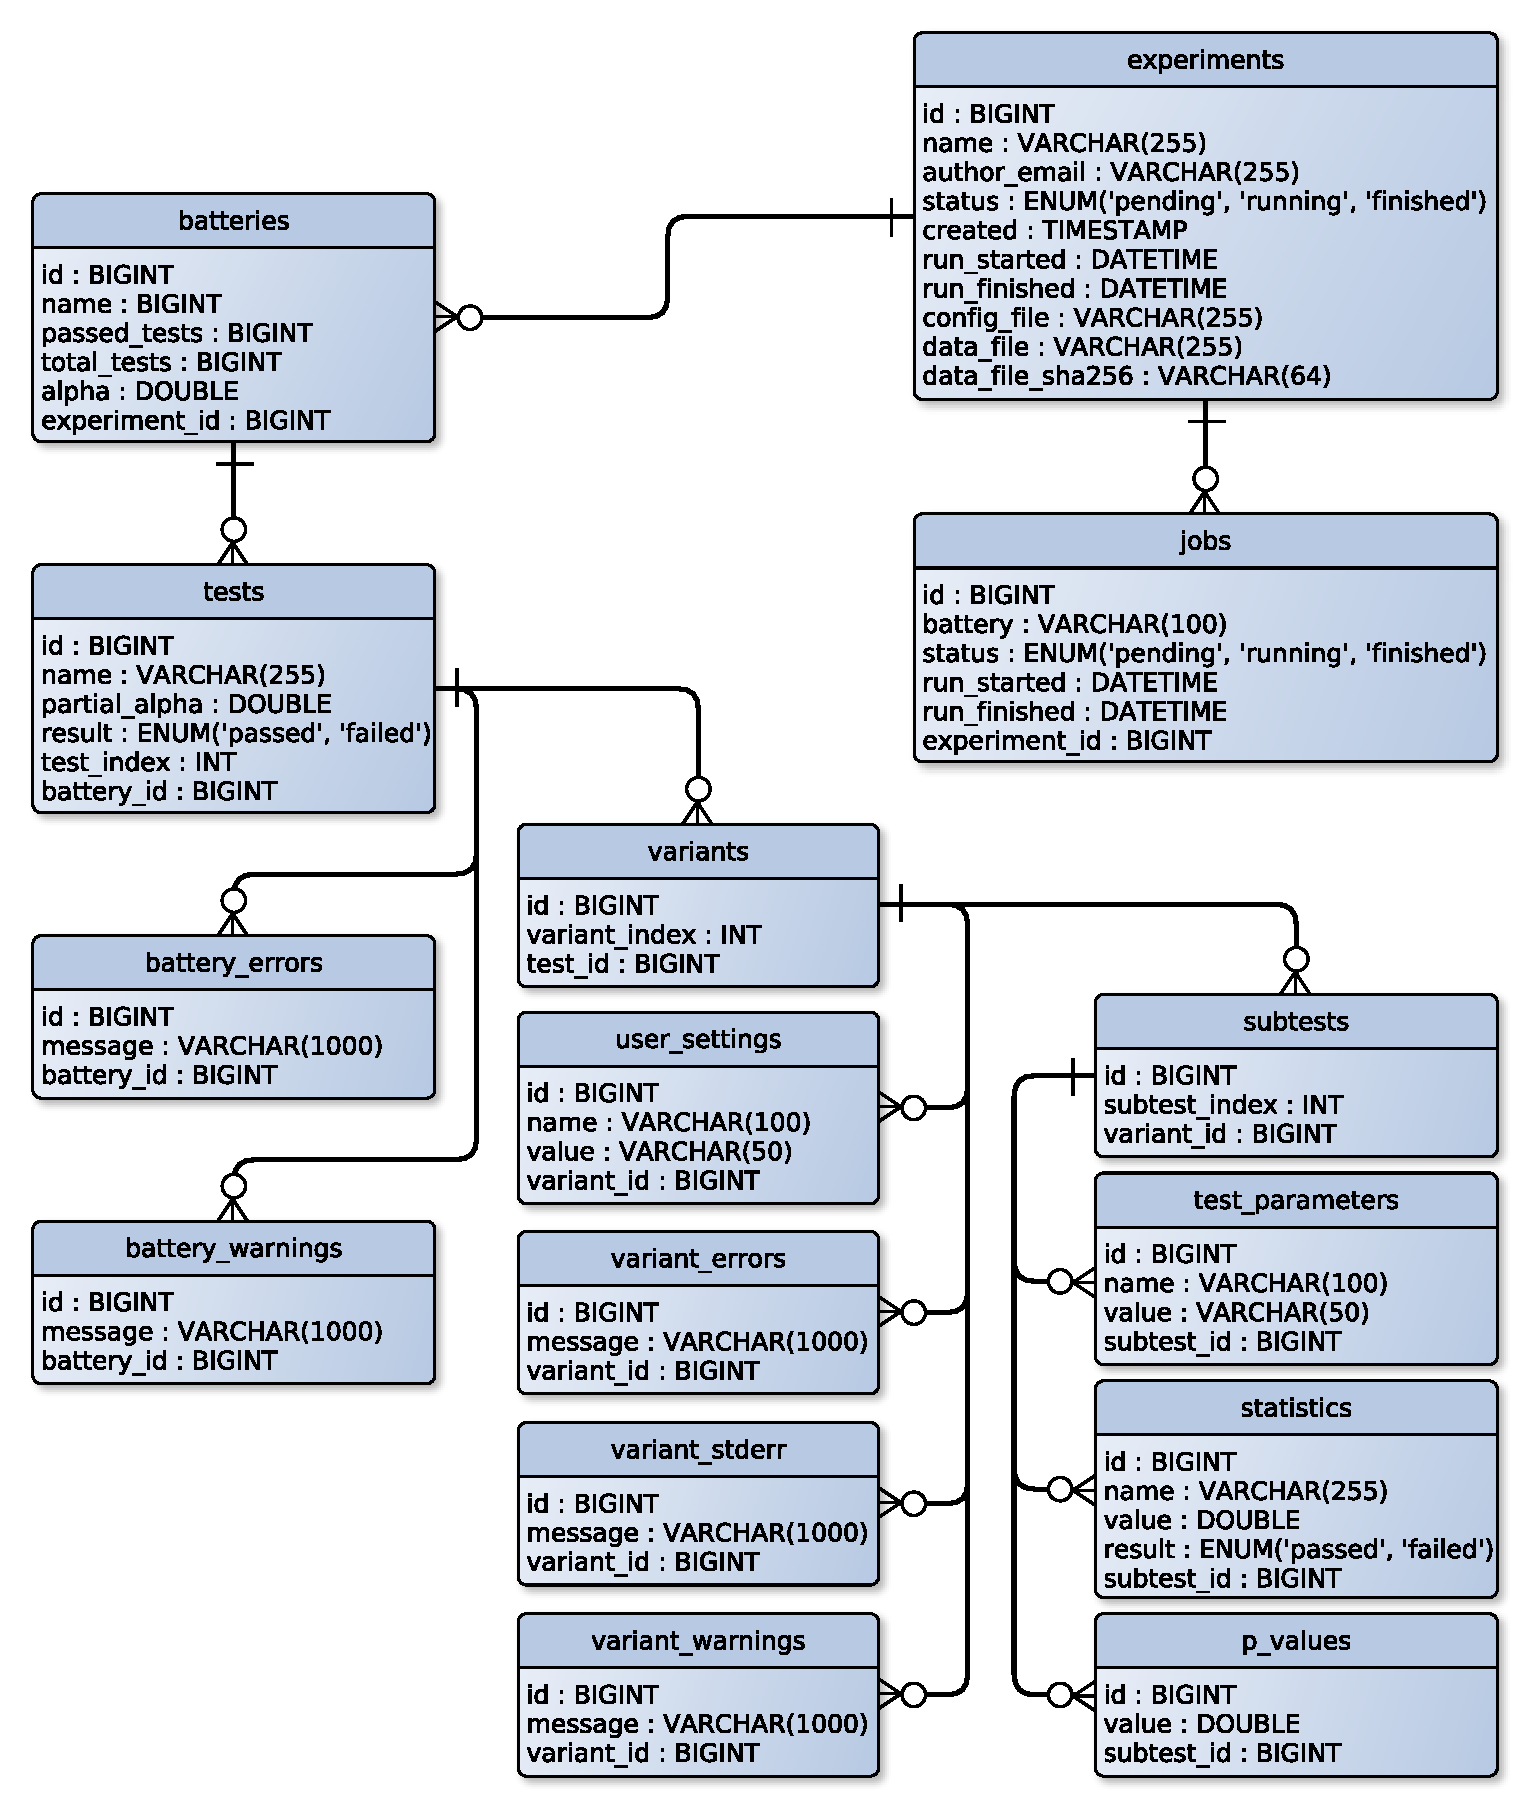
\includegraphics[width=\paperwidth-3.5cm]{figures/database-erd-model.pdf}
\end{nomar}
\caption{ERD Model of the database}
\label{fig:erd_database}
\end{figure}

\section{Remote access to RTT}
Remote access to RTT allows the users to perform the binary data analysis without the need for the installation of the toolkit and without execution of the tool on their local machine. The statistical testing is, in certain configurations, demanding on computational time and resources. Having the RTT installed on remote machines allows us to scale the resources available for the toolkit and further speed-up the analysis. The user only needs to provide the data for the toolkit and choose (or provide his own) configuration for the batteries. After the testing, the user is notified and can inspect the results.

In the deployment part of the project, we developed an utility project that handles setup and installation of the local interface on single or multiple machines. The deployment project also handles setup of auxiliary scripts and tools that are required for result database and data storage and that will be used by the machines used for statistical testing computation. The database and storage can be deployed on separate machines or on single server that will handle all of the tasks along with the computation of the results. 

The interaction of the user with the infrastructure is visualized in Figure~TODO. In following section we outline the different purposes of the servers.

\subsection{Database server}
The machine hosting MySQL server with created database for RTT as shown in Figure~\ref{fig:erd_database}. The database is used for storing the results of the analyses as well as information used for scheduling and distribution of jobs to backend servers.

\subsection{Storage server}
The server hosts a storage space that acts as a temporary deposit for the data that is not yet distributed and analysed on the backend servers. After the distribution and analysis, the data is removed from the machine.

\begin{titlemize}{Scripts on the server}
\item \texttt{clean\_cache.py} -- Script that handles removal of the data files that were already analysed. The script is executed periodically.
\end{titlemize}

\subsection{Backend server}
Single or multiple machines that host installed toolkit and batteries. The analysis of the data is executed on these machines. If there are multiple backend servers, the analyses are scheduled based on the information stored in the database. Prior to the analysis, the data is downloaded from the storage and stored in local cache. After the computation, the results are stored on the database server and the data is deleted.

Both jobs and experiments can be in one of the three states -- \texttt{pending}, \texttt{running} and \texttt{finished}; the descriptions of the states are in Table~\ref{tab:states_jobs_exps}. Scheduling of the computation is based on the state of the experiments and jobs.

\begin{table}[h!]
\begin{nomar}
\centering
\begin{tabular}{l || p{4cm} | p{4cm}}
\textbf{Status}   & \textbf{Job} & \textbf{Experiment} \\ \hline \hline
\texttt{pending}  & The job is waiting for execution. & All of the jobs related to the experiment are waiting for execution. \\ \hline
\texttt{running}  & The job is being \newline executed on backend server. & Some or all related jobs are being \newline executed. \\ \hline
\texttt{finished} & The jobs execution ended. & The execution of all \newline related jobs ended. \\
\end{tabular}
\end{nomar}
\caption{States of jobs and experiments}
\label{tab:states_jobs_exps}
\end{table}

\begin{titlemize}{Scripts on the server}
\item \texttt{clean\_cache.py} -- Script that handles removal of the locally cached data files that were already analysed. The script is executed periodically.
\item \texttt{run\_jobs.py} -- Script responsible for choosing the correct computational job, downloading the data from the storage server and the execution of the analysis. Th script is executed periodically. The jobs are picked from the database table \texttt{jobs} with following priority:
\begin{enumerate}
\item Jobs of those experiments whose data was downloaded earlier and the data is present in the local cache of the server.
\item Any jobs of the experiments that are in pending state.
\item Any jobs that are in pending state.
\end{enumerate}
The rules are designed in such a way that a minimal amount of data is transferred over the network. If there are enough distinct pending experiments for all servers then each server will pick single experiment and execute all its jobs and the data of the experiment is transferred only once.
\end{titlemize}

\subsection{Frontend server}
The frontend server is the only server that the user directly interacts with. The machine accepts data and request for creating an experiment. After the request, the server creates the experiment and related jobs in the database and uploads the data into the storage.

The server can be accessed either via SSH, which is intended for experienced users or via web interface which is intuitive and user-friendly.

\subsection{Access via web browser}
The web browser interface is intended to accomodate the needs of common users. The main idea is that the user will visit our website and, using the interface, will create his experiment. For basic testing the user is only required to upload the data and suitable battery will be chosen for him. Alternatively he can also choose the desired configuration or create his own documentation from the scratch. The results of the analysis are also shown in the interface. 

This approach is not intended to be used for creating big amount of experiments.

\subsection{SSH}
The direct access to the frontend server is meant for advanced users that need to analyze big volumes of data. Upon request, the user is able to gain direct access to separated part of the system on the frontend machine. The separated system contains only tools that allows him to create experiments for RTT. The data for the testing can be uploaded from the users local machine, downloaded from another server using sftp or generated right on the frontend server. The tool that can be used for stream generation was developed at CRoCS and is capable of producing outputs of numerous cryptographic primitives. The settings of the generator provide high control of the output to the user. 

\section{Result interpretation}
\begin{huge}
todo
\end{huge}

\chapter{Analysis of outputs of cryptographic functions, comparison with EACirc}
\begin{itemize}
\item How the data were tested
\item List functions
\item List interesting (differing) results - Dieharder, NIST STS, TestU01, EACirc, polynomials(???)
\end{itemize}

\chapter{Analysis of DIEHARDER results on quantum random data}
\begin{itemize}
\item Statistical intro, uniformity, first vs. second level p-value, etc...
\item Two experiments - continuous p-values, blocks of 2nd level
\item Results - non-uniform, where it will begin to show on 2nd level results
\end{itemize}

\chapter{Conclusions}
\begin{itemize}
\item Developed user-friendly tool for easy analysis of arbitrary binary data - Randomness Testing Toolkit
\item Interpretation of results
\item Comparison of batteries with EACirc, polynomials
\item Defects in Dieharder, their relevance, etc...
\item Future work, same analysis on TestU01, dependence between tests(?), continuous development of RTT, call for flawless statistical battery ( :) )
\end{itemize}

\appendix

\printbibliography

\chapter{Sample file with RTT settings}
\label{app:rtt_sett_json}
\begin{minted}[mathescape,
               linenos,
               numbersep=5pt,
               gobble=2,
               frame=lines,
               framesep=2mm]{json}
  {
    "toolkit-settings": {
      "logger": {
        "dir-prefix": "rtt-results/logs",
        "run-log-dir": "run-logs",
        "dieharder-dir": "dieharder",
        "nist-sts-dir": "niststs",
        "tu01-smallcrush-dir": "testu01/smallcrush",
        "tu01-crush-dir": "testu01/crush",
        "tu01-bigcrush-dir": "testu01/bigcrush",
        "tu01-rabbit-dir": "testu01/rabbit",
        "tu01-alphabit-dir": "testu01/alphabit",
        "tu01-blockalphabit-dir": "testu01/blockalphabit"
      },
      "result-storage": {
        "file": {
          "main-file": "rtt-results/table.txt",
          "dir-prefix": "rtt-results/reports",
          "dieharder-dir": "dieharder",
          "nist-sts-dir": "niststs",
          "tu01-smallcrush-dir": "testu01/smallcrush",
          "tu01-crush-dir": "testu01/crush",
          "tu01-bigcrush-dir": "testu01/bigcrush",
          "tu01-rabbit-dir": "testu01/rabbit",
          "tu01-alphabit-dir": "testu01/alphabit",
          "tu01-blockalphabit-dir": "testu01/blockalphabit"
        },
        "mysql-db": {
          "address": "127.0.0.1",
          "port": "3306",
          "name": "rtt",
          "credentials-file": "credentials.json"
        }
      },
      "binaries": {
        "nist-sts": "/home/rtt-statistical-batteries/nist-sts",
        "dieharder": "/home/rtt-statistical-batteries/dieharder",
        "testu01": "/home/rtt-statistical-batteries/testu01"
      },
      "miscelaneous": {
        "nist-sts": {
          "main-result-dir": "experiments/AlgorithmTesting/"
        }
      },
      "execution": {
        "max-parallel-tests": 8,
        "test-timeout-seconds": 3600
      }
    }
  }
\end{minted}

\chapter{Example of file storage report file}
\label{app:file_storage_report}
\begin{minted}{text}
***** Randomness Testing Toolkit data stream analysis report *****
Date:    05-04-2017
File:    data.bin
Battery: Dieharder

Alpha:   0.01
Epsilon: 1e-08

Passed/Total tests: 1/1

Battery errors:

Battery warnings:


-----------------------------------------------------------
Diehard Runs Test test results:
    Result: Passed
    Test partial alpha: 0.00250943

    Variant 1:
        User settings: 
            P-sample count: 10
        ************

        Subtest 1:
            Kolmogorov-Smirnov statistic p-value: 0.78507772 Passed
            p-values: 
                0.05899849 0.14303914 0.25813353 0.26205674 0.29277325 
                0.35258302 0.56733382 0.65239775 0.72661662 0.97024989 
            ============
        ############

        Subtest 2:
            Kolmogorov-Smirnov statistic p-value: 0.98126677 Passed
            p-values: 
                0.06708958 0.13845018 0.24143043 0.30884227 0.34883845 
                0.45856887 0.50099963 0.72226328 0.79368168 0.94420838 
            ============
        ############

    ^^^^^^^^^^^^

    Variant 2:
        User settings: 
            P-sample count: 20
        ************

        Subtest 1:
            Kolmogorov-Smirnov statistic p-value: 0.94522158 Passed
            p-values: 
                0.02636030 0.05899849 0.07020394 0.11462969 0.14303914 
                0.25813353 0.26205674 0.29277325 0.35258302 0.42201984 
                0.49409172 0.50249791 0.50852031 0.56733382 0.65239775 
                0.72661662 0.87379533 0.94805962 0.95109797 0.97024989 
            ============
        ############

        Subtest 2:
            Kolmogorov-Smirnov statistic p-value: 0.97098651 Passed
            p-values: 
                0.05940416 0.06708958 0.10176118 0.13845018 0.18591525 
                0.20171335 0.24143043 0.30884227 0.34883845 0.45856887 
                0.47711566 0.50099963 0.51679868 0.57821548 0.72226328 
                0.73270941 0.79368168 0.91155189 0.94420838 0.99216956 
            ============
        ############

    ^^^^^^^^^^^^

-----------------------------------------------------------
\end{minted}

\end{document}
